%---------------------------------------------------------

\begin{frame}{Relacja płotkowania}


\begin{columns}[c,onlytextwidth]
  % LABELS
  \begin{column}{0.2\textwidth}
      
  \end{column}
  \begin{column}{0.15\textwidth} 
  \vspace{-3.5em}\\
    $F_1(u,v) \equiv$

    \vspace{4em}

    $F_2(u,v) \equiv$

    \vspace{5em}

    $F_3(u,v) \equiv$
  \end{column}

  \begin{column}{0.82\textwidth}
    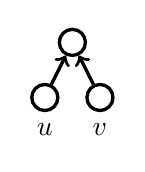
\begin{tikzpicture}[
    scale=0.35,
    line width=1.2pt
]

    % \node at (-3,-5.5) {\(F_1\)};
    
    \node[circle, draw=black, fill=white, label=below:{\(u\)}]
            (p0) at (-4,-4) {};

    \node[circle, draw=black, fill=white, label=below:{\(v\)}]
            (p1) at (-2,-4) {};

    \node[circle, draw=black, fill=white]
        (p2) at (-3,-2) {};
    

    \draw[->] (p0) -- (p2);
    \draw[->] (p1) -- (p2);
\end{tikzpicture}

    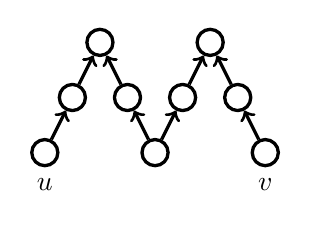
\begin{tikzpicture}[
    scale=0.35,
    line width=1.2pt
]
   % \node at (-4,-2) {\(F_2\)};
            
    \node[circle, draw=black, fill=white, label=below:{\(u\)}]
            (q0) at (4,-4) {};
    \node[circle, draw=black, fill=white, label=below:{}]
            (q1) at (8,-4) {};
    \node[circle, draw=black, fill=white, label=below:{\(v\)}]
            (q2) at (12,-4) {};
    \node[circle, draw=black, fill=white, label=below:{}]
            (q3) at (5,-2) {};
    \node[circle, draw=black, fill=white, label=below:{}]
            (q4) at (7,-2) {};
    \node[circle, draw=black, fill=white, label=below:{}]
            (q5) at (9,-2) {};
    \node[circle, draw=black, fill=white, label=below:{}]
            (q6) at (11,-2) {};
    \node[circle, draw=black, fill=white, label=below:{}]
        (q7) at (6,0) {};
    \node[circle, draw=black, fill=white, label=below:{}]
        (q8) at (10,0) {};   
        
    \draw[->] (q0) -- (q3);
    \draw[->] (q3) -- (q7);
    \draw[->] (q4) -- (q7);
    \draw[->] (q1) -- (q4);
    \draw[->] (q1) -- (q5);
    \draw[->] (q2) -- (q6);
    \draw[->] (q5) -- (q8);
    \draw[->] (q6) -- (q8);
\end{tikzpicture}

    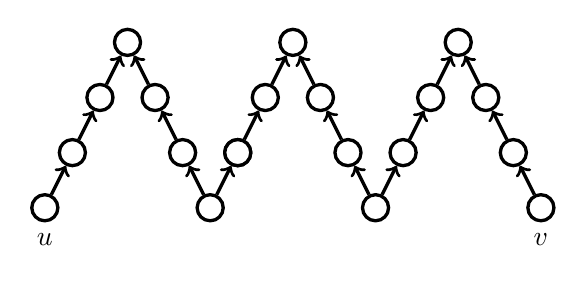
\begin{tikzpicture}[
    scale=0.35,
    line width=1.2pt
]
    % \node at (-7,-10) {\(F_3\)};
            
    \node[circle, draw=black, fill=white, label=below:{\(u\)}]
            (r0) at (-4,-13) {};
    \node[circle, draw=black, fill=white, label=below:{}]
            (r1) at (2,-13) {};
    \node[circle, draw=black, fill=white, label=below:{}]
            (r2) at (8,-13) {};
    \node[circle, draw=black, fill=white, label=below:{\(v\)}]
            (r3) at (14,-13) {};
    \node[circle, draw=black, fill=white, label=below:{}]
            (r4) at (-3,-11) {};
    \node[circle, draw=black, fill=white, label=below:{}]
            (r5) at (1,-11) {};
    \node[circle, draw=black, fill=white, label=below:{}]
            (r6) at (3,-11) {};
    \node[circle, draw=black, fill=white, label=below:{}]
            (r7) at (7,-11) {};
    \node[circle, draw=black, fill=white, label=below:{}]
            (r8) at (9,-11) {};
    \node[circle, draw=black, fill=white, label=below:{}]
            (r9) at (13,-11) {};
    \node[circle, draw=black, fill=white, label=below:{}]
            (r10) at (3,-11) {};
    \node[circle, draw=black, fill=white, label=below:{}]
            (r11) at (-2,-9) {};
    \node[circle, draw=black, fill=white, label=below:{}]
            (r12) at (0,-9) {};
    \node[circle, draw=black, fill=white, label=below:{}]
            (r13) at (4,-9) {};
    \node[circle, draw=black, fill=white, label=below:{}]
            (r14) at (6,-9) {};
    \node[circle, draw=black, fill=white, label=below:{}]
            (r15) at (10,-9) {};
    \node[circle, draw=black, fill=white, label=below:{}]
            (r16) at (12,-9) {};
    \node[circle, draw=black, fill=white, label=below:{}]
            (r17) at (-1,-7) {};
    \node[circle, draw=black, fill=white, label=below:{}]
            (r18) at (5,-7) {};
    \node[circle, draw=black, fill=white, label=below:{}]
            (r19) at (11,-7) {};

    \draw[->] (r0) -- (r4);
    \draw[->] (r1) -- (r5);
    \draw[->] (r1) -- (r6);
    \draw[->] (r2) -- (r7);
    \draw[->] (r2) -- (r8);
    \draw[->] (r3) -- (r9);
    \draw[->] (r4) -- (r11);
    \draw[->] (r5) -- (r12);
    \draw[->] (r6) -- (r13);
    \draw[->] (r7) -- (r14);
    \draw[->] (r8) -- (r15);
    \draw[->] (r9) -- (r16);
    \draw[->] (r11) -- (r17);
    \draw[->] (r12) -- (r17);
    \draw[->] (r13) -- (r18);
    \draw[->] (r14) -- (r18);
    \draw[->] (r15) -- (r19);
    \draw[->] (r16) -- (r19);
\end{tikzpicture}
  \end{column}
\end{columns}

\end{frame}
%---------------------------------------------------------


\begin{frame}{Stabilizacja płotków}
    \begin{figure}
        \centering
        \only<1-3>{
\begin{tikzpicture}[
    scale=0.5,
    line width=1.2pt
]

            
    \node[circle, draw=black, fill=white, label=below:{\(u\)}]
            (q0) at (4,-4) {};
    \node[circle, draw=black, fill=white, label=below:{}]
            (q1) at (8,-4) {};
    \node[circle, draw=black, fill=white, label=below:{\(v\)}]
            (q2) at (12,-4) {};
    \node[circle, draw=black, fill=white, label=below:{}]
            (q3) at (5,-2) {};
    \node[circle, draw=black, fill=white, label=below:{}]
            (q4) at (7,-2) {};
    \node[circle, draw=black, fill=white, label=below:{}]
            (q5) at (9,-2) {};
    \node[circle, draw=black, fill=white, label=below:{}]
            (q6) at (11,-2) {};
    \node[circle, draw=black, fill=white, label=left:{}]
        (q7) at (6,0) {};
    \node[circle, draw=black, fill=white, label=left:{}]
        (q8) at (10,0) {}; 
    
        
    \draw[->] (q0) -- (q3);
    \draw[->] (q3) -- (q7);
    \draw[->] (q4) -- (q7);
    \draw[->] (q1) -- (q4);
    \draw[->] (q1) -- (q5);
    \draw[->] (q2) -- (q6);
    \draw[->] (q5) -- (q8);
    \draw[->] (q6) -- (q8);


\onslide<2->{
    \node[circle, draw=cfnavy, fill=white, label=below:{}]
        (q9) at (6,2) {};  
    \node[circle, draw=cfnavy, fill=white, label=below:{}]
        (q10) at (10,2) {}; 
    \draw[->] (q7) -- (q9);
    \draw[->] (q8) -- (q10);
}

\onslide<3>{
    \node[circle, draw=cfnavy, fill=white, label=below:{}]
        (q11) at (12,-2) {};  
    \node[circle, draw=cfnavy, fill=white, label=below:{}]
        (q12) at (12,0) {};
    \node[circle, draw=cfnavy, fill=white, label=below:{}]
        (q13) at (12,2) {};
    \draw[->] (q2) -- (q11);
    \draw[->] (q11) -- (q12);
    \draw[->] (q12) -- (q13);
}
    
\end{tikzpicture}
}
        \only<4->{
\begin{tikzpicture}[
    scale=0.5,
    line width=1.2pt
]

            
    \node[circle, draw=black, fill=white, label=below:{\(u\)}]
            (r0) at (-4,-13) {};
    \node[circle, draw=black, fill=white, label=below:{}]
            (r1) at (2,-13) {};
    \node[circle, draw=black, fill=white, label=below:{\(v\)}]
            (r2) at (8,-13) {};
    \node[circle, draw=black, fill=white, label=below:{\(v\)}]
            (r3) at (14,-13) {};
    \node[circle, draw=black, fill=white, label=below:{}]
            (r4) at (-3,-11) {};
    \node[circle, draw=black, fill=white, label=below:{}]
            (r5) at (1,-11) {};
    \node[circle, draw=black, fill=white, label=below:{}]
            (r6) at (3,-11) {};
    \node[circle, draw=black, fill=white, label=below:{}]
            (r7) at (7,-11) {};
    \node[circle, draw=cfpink, fill=white, label=right:{\(r_4\)}]
            (r8) at (9,-11) {};
    \node[circle, draw=cfpink, fill=white, label=right:{\(r_4\)}]
            (r9) at (13,-11) {};
    \node[circle, draw=black, fill=white, label=below:{}]
            (r10) at (3,-11) {};
    \node[circle, draw=cfgr, fill=white, label=left:{\(r_1\)}]
            (r11) at (-2,-9) {};
    \node[circle, draw=cfgr, fill=white, label=right:{\(r_1\)}]
            (r12) at (0,-9) {};
    \node[circle, draw=cfred, fill=white, label=left:{\(r_2\)}]
            (r13) at (4,-9) {};
    \node[circle, draw=cfred, fill=white, label=right:{\(r_2\)}]
            (r14) at (6,-9) {};
    \node[circle, draw=cfyel, fill=white, label=left:{\(r_3\)}]
            (r15) at (10,-9) {};
    \node[circle, draw=cfyel, fill=white, label=right:{\(r_3\)}]
            (r16) at (12,-9) {};
    \node[circle, draw=cfnavy, fill=white, label=below:{}]
            (r17) at (-1,-7) {};
    \node[circle, draw=cfnavy, fill=white, label=below:{}]
            (r18) at (5,-7) {};
    \node[circle, draw=cfnavy, fill=white, label=below:{}]
            (r19) at (11,-7) {};

    \draw[->] (r0) -- (r4);
    \draw[->] (r1) -- (r5);
    \draw[->] (r1) -- (r6);
    \draw[->] (r2) -- (r7);
    \draw[->] (r2) -- (r8);
    \draw[->] (r3) -- (r9);
    \draw[->] (r4) -- (r11);
    \draw[->] (r5) -- (r12);
    \draw[->] (r6) -- (r13);
    \draw[->] (r7) -- (r14);
    \draw[->] (r8) -- (r15);
    \draw[->] (r9) -- (r16);
    \draw[->] (r11) -- (r17);
    \draw[->] (r12) -- (r17);
    \draw[->] (r13) -- (r18);
    \draw[->] (r14) -- (r18);
    \draw[->] (r15) -- (r19);
    \draw[->] (r16) -- (r19);

    % \draw[dashed] (r2) -- (r3) node[midway, above]{};
    % \draw[dashed] (r8) -- (r9) node[midway, above]{};
    % \draw[dashed] (r15) -- (r16) node[midway, above]{};
    % \draw[dashed] (r11) -- (r12) node[midway, above]{};
    % \draw[dashed] (r13) -- (r14) node[midway, above]{};
    
\end{tikzpicture}
}
    \end{figure}
    Jeśli istnieje płotek \(F_n(u,v)\), to istnieje także płotek \(F_{n+1}(u,v)\).
    \\
    \vspace{1em}
    \onslide<5>{
    Od pewnego momentu relacja się ustabilizuje: \vspace{-1em}
    \[ F_1 \subseteq F_2 \subseteq F_3 \subseteq \dots \subseteq F_m = F \]
    }
\end{frame}